% !TeX program = pdflatex
% Sprawozdanie projektu "Football tracker"
% Przedmiot: Analiza i Przetwarzanie Obrazow
% Kompilacja: pdflatex sprawozdanie.tex (dwukrotnie, dla spisu tresci)

\documentclass[11pt,a4paper]{article}

\usepackage{iftex}
\ifPDFTeX
  \usepackage[utf8]{inputenc}
  \usepackage[T1]{fontenc}
  \usepackage{lmodern}
\else
  \usepackage{fontspec}
\fi
\usepackage[polish]{babel}
\usepackage{amsmath}
\usepackage[a4paper,margin=2.4cm]{geometry}
\usepackage{graphicx}
\usepackage{float}
\usepackage{booktabs}
\usepackage{array}
\usepackage{xcolor}
\usepackage{listings}
\usepackage{enumitem}
\usepackage{caption}
\usepackage[hidelinks]{hyperref}

\graphicspath{{img/}}

% --- styl listingow kodu ---
\definecolor{codebg}{rgb}{0.97,0.97,0.97}
\definecolor{codekw}{rgb}{0.13,0.29,0.53}
\definecolor{codecm}{rgb}{0.40,0.50,0.40}
\definecolor{codestr}{rgb}{0.55,0.20,0.10}

\lstdefinestyle{py}{
  language=Python,
  backgroundcolor=\color{codebg},
  basicstyle=\ttfamily\scriptsize,
  keywordstyle=\color{codekw}\bfseries,
  commentstyle=\color{codecm}\itshape,
  stringstyle=\color{codestr},
  numbers=left,
  numberstyle=\tiny\color{gray},
  numbersep=7pt,
  showstringspaces=false,
  breaklines=true,
  frame=single,
  framesep=4pt,
  rulecolor=\color{gray!40},
  captionpos=b,
  tabsize=2,
  literate={ł}{{\l}}1 {Ł}{{\L}}1
}

\lstdefinestyle{sh}{
  backgroundcolor=\color{codebg},
  basicstyle=\ttfamily\footnotesize,
  breaklines=true,
  frame=single,
  framesep=4pt,
  rulecolor=\color{gray!40},
  tabsize=2
}

\captionsetup{font=small,labelfont=bf}
\setlength{\parskip}{0.5em}
\setlength{\parindent}{0pt}

% =====================================================================
\begin{document}

% --------------------------- STRONA TYTULOWA ---------------------------
\begin{titlepage}
\centering
\vspace*{2.5cm}

{\Large\scshape Analiza i Przetwarzanie Obrazów}

\vspace{0.5cm}
{\Huge\bfseries Football tracker}

\vspace{0.5cm}
{\large Detekcja i śledzenie zawodników na nagraniach meczów piłkarskich}

\vspace{0.4cm}
\rule{\linewidth}{0.5pt}

\vspace{1.5cm}
{\large\itshape Sprawozdanie z projektu}

\vspace{3cm}
{\large\bfseries Autorzy:}

Bartłomiej Obrochta \\
Kamil Milewski \\
Maciej Leśniak \\

\vfill
{\large \today}

\end{titlepage}

% --------------------------- SPIS TRESCI ---------------------------
\tableofcontents
\newpage

% =====================================================================
\section{Temat i założenia projektu}

Celem projektu \textbf{Football tracker} jest stworzenie kompletnego potoku
przetwarzania obrazu, który na podstawie nagrania meczu piłkarskiego
automatycznie wykrywa zawodników (w tym osobno bramkarzy), sędziów i piłkę, śledzi ich pomiędzy
kolejnymi klatkami, a następnie rzutuje ich pozycje na schematyczny widok
boiska z lotu ptaka (minimapę 2D) i wylicza proste statystyki, takie
jak pokonany dystans i prędkość poszczególnych zawodników.

Projekt obejmuje:
\begin{itemize}[nosep]
  \item detekcję zawodników, piłki i sędziów,
  \item trwałe śledzenie tożsamości (ID) obiektów pomiędzy klatkami, czyli wyznaczanie trajektorii,
  \item odwzorowanie ramek otaczających (\emph{bounding boxów}) na widok boiska z góry,
  \item wyznaczanie homografii \emph{per klatka} na podstawie wyuczonych
        punktów charakterystycznych boiska,
  \item obliczanie pokonanego dystansu i prędkości każdego zawodnika,
  \item potok wsadowy (\texttt{process.py}) generujący gotowy plik wideo wraz z
        tabelą podsumowującą oraz dwuetapowy schemat trenowania modelu boiska.
\end{itemize}

Architektura potoku jest dwumodelowa i przebiega następująco:
\[
\begin{aligned}
  &\text{YOLO26 (detektor)} \rightarrow \text{ByteTrack (tracking)} \rightarrow \\
  &\text{YOLO26-pose (32 keypointy boiska)} \rightarrow \text{homografia} \rightarrow \\
  &\text{minimapa 2D} + \text{dystans/prędkość}.
\end{aligned}
\]

Dwoma trenowanymi komponentami są: \textbf{detektor obiektów} (zawodnik,
bramkarz, sędzia, piłka) oraz \textbf{model punktów charakterystycznych boiska}
(model typu \emph{pose} z 32 punktami). Komponenty śledzące (ByteTrack) oraz
moduł homografii nie są uczone -- są to klasyczne algorytmy (filtr Kalmana +
algorytm węgierski w trackerze, RANSAC w homografii).

% =====================================================================
\section{Zbiory danych}
\label{sec:dane}

Projekt korzysta z czterech zbiorów danych. Dwa z nich służą do uczenia
detektora zawodników, a dwa -- do uczenia modelu punktów boiska. Co istotne,
katalogi z danymi pobiera się skryptem \texttt{dataset.py}.

\subsection{Zbiory do detekcji zawodników (4 klasy)}

Schemat klas jest wspólny dla obu źródeł detekcyjnych i zdefiniowany w pliku
\texttt{configs/classes.yaml}:

\begin{center}
\begin{tabular}{cl}
\toprule
ID & Klasa \\
\midrule
0 & player (zawodnik z pola) \\
1 & goalkeeper (bramkarz) \\
2 & referee (sędzia) \\
3 & ball (piłka) \\
\bottomrule
\end{tabular}
\end{center}

\textbf{Roboflow Players} -- zbiór \texttt{football-players-detection-3zvbc}
(wersja~12) z platformy Roboflow Universe. Zawiera pojedyncze klatki z nagrań
meczowych, na których obiekty (zawodnicy, bramkarze, sędziowie, piłka) są
opisane prostokątnymi ramkami otaczającymi (ok.~600
klatek). Zbiór jest udostępniany od razu w formacie YOLO; pobierany jest w
formacie \texttt{yolov8}. Etykiety oryginalne mają inną kolejność klas, dlatego
po pobraniu są przemapowywane do schematu kanonicznego
(\texttt{ball$\rightarrow$3, goalkeeper$\rightarrow$1, player$\rightarrow$0,
referee$\rightarrow$2}).

\textbf{SoccerNet Tracking} -- opcjonalny, większy zbiór z projektu SoccerNet
(dostęp po zaakceptowaniu NDA i podaniu hasła). Zawiera sekwencje klatek z
meczów z adnotacjami w stylu MOT (\texttt{gt.txt}: numer klatki, ID obiektu,
pozycja ramki, klasa). W projekcie dane są konwertowane do formatu YOLO, a klasy
przemapowywane (\texttt{1$\rightarrow$player, 2$\rightarrow$goalkeeper,
3$\rightarrow$referee, 4$\rightarrow$ball}). Heurystyka podziału: klipy ze słowem
\texttt{test} w ścieżce trafiają do zbioru walidacyjnego, pozostałe do
treningowego.

Oba zbiory detekcyjne łączone są poleceniem \texttt{python dataset.py merge} do
katalogu \texttt{data/processed/combined/} (z prefiksami \texttt{soccernet\_\_}
oraz \texttt{roboflow\_\_}), co generuje plik \texttt{configs/combined.yaml}
używany w treningu i ewaluacji detektora.

\subsection{Zbiory do detekcji punktów boiska (1 klasa + 32 keypointy)}

Model boiska to model typu \emph{pose}: wykrywa jedną ramkę klasy
\texttt{pitch} (cały widoczny obszar boiska) oraz 32 punkty charakterystyczne.
Kanoniczny schemat 32 punktów (w metrach, dla boiska FIFA $105 \times 68$~m) jest
zdefiniowany w \texttt{configs/pitch\_keypoints.yaml} i obejmuje m.in.: cztery
rogi boiska, końce linii środkowej, narożniki pól karnych i bramkowych, punkty
przy słupkach, punkt środkowy, punkty karne oraz wierzchołek łuku pola karnego.

\textbf{Roboflow Pitch} -- zbiór \texttt{football-field-detection-f07vi}
(wersja~15). Zawiera obrazy boiska, najczęściej w szerokich ujęciach taktycznych,
z naniesionymi 32 punktami charakterystycznymi w formacie YOLO-pose. Według
dokumentacji ok.~317 klatek. Pobierany jest w formacie \texttt{yolo26}, a do
\texttt{data.yaml} wstrzykiwane są pola \texttt{kpt\_shape: [32, 3]} oraz
\texttt{flip\_idx} (mapa odbicia lustrzanego punktów lewa/prawa strona boiska).

\textbf{SoccerNet Calibration 2023} -- zbiór do kalibracji geometrii boiska
(ok.~13~tys.\ klatek broadcastowych). Nie zawiera ramek zawodników; zawiera
adnotacje \emph{linii} boiska. Projekt przelicza te linie na 32 punkty -- przez
wyznaczanie przecięć par linii (np. linia boczna $\cap$ linia bramkowa = róg
boiska). Punkty 28--31 (punkt środkowy, punkty karne, wierzchołek łuku) nie
występują w adnotacjach SoccerNet i pozostają niewidoczne dla tego źródła.

\subsection{Łączenie i wstępne przetwarzanie zbioru boiska}

Po pobraniu obu źródeł boiska są one łączone i poddawane \emph{green
suppression} -- tłumieniu kanału zielonego, dzięki czemu białe linie boiska
stają się bardziej wyraziste względem trawy. Tę samą operację stosuje się
identycznie podczas uczenia i podczas wnioskowania, co zapewnia spójność cech.
Jej implementacja jest bardzo zwięzła (Listing~\ref{lst:green}).

\begin{lstlisting}[style=py,caption={Tłumienie kanału zielonego -- \texttt{src/football\_tracker/pitch/preprocess.py}},label={lst:green}]
def enhance_pitch_lines(frame: np.ndarray, green_factor: float = 0.75) -> np.ndarray:
    """Suppress the green channel to make white pitch lines stand out.
    Grass pixels have G >> R,B.  White lines have R~=G~=B (high brightness).
    Multiplying the G channel by < 1 darkens grass without affecting lines."""
    out = frame.astype(np.float32)
    out[:, :, 1] *= green_factor          # suppress green
    return np.clip(out, 0, 255).astype(np.uint8)
\end{lstlisting}

Wynikowy zbiór (\texttt{data/processed/combined\_pitch\_gs/}) liczy 
 ok.~13,3~tys.\ obrazów treningowych i ok.~2,5~tys.\ walidacyjnych,
przy czym zachowywane są tylko etykiety z co najmniej 4 widocznymi punktami
(4~to geometryczne minimum do wyznaczenia homografii).

\subsection{Augmentacja offline modelu boiska}

Wbudowana augmentacja YOLO dobrze radzi sobie z geometrią, ale słabo z
różnorodnością fotometryczną oraz z kadrami pokazującymi tylko część boiska.
Ponieważ wszystkie klatki źródłowe pokazują całe boisko, model uczy się np.,
że „linia środkowa $\approx$ 50\% szerokości obrazu”, a następnie myli punkty
przy zbliżeniach na jedną połowę. Rozwiązuje to augmentacja \emph{offline}
(moduł \texttt{augment\_pitch\_dataset.py}, wymaga biblioteki
\texttt{albumentations}), która dla każdego obrazu źródłowego zapisuje na dysk:
\begin{itemize}[nosep]
  \item 1 dowiązanie do oryginału,
  \item 2 kopie z augmentacją fotometryczną (jasność/kontrast, HSV, gamma,
        CLAHE, rozmycie, szum, kompresja JPEG, sporadycznie skala szarości,
        wycinanie fragmentów oraz drobne przekształcenia geometryczne),
  \item \textbf{11 strategicznych wycinków} fragmentów boiska (połówki,
        ćwiartki, środek, zbliżenia na pola bramkowe) -- każdy także
        augmentowany fotometrycznie.
\end{itemize}
Daje to do ok.~14 próbek na obraz źródłowy, czyli ok.~110~tys.\ obrazów
treningowych. Próbki, w których po przekształceniu zostaje mniej niż 4 widoczne
punkty, są odrzucane. Zbiór walidacyjny domyślnie nie jest augmentowany (aby
metryki pozostały porównywalne). Tryb \texttt{--partials-only} zapisuje wyłącznie
11 wycinków na obraz (ok.~80~tys.\ obrazów) i służy do etapu dostrajania.

\subsection{Opcje skryptu \texttt{dataset.py}}

\begin{center}
\small
\begin{tabular}{>{\ttfamily}l p{6.3cm} >{\ttfamily\footnotesize}l}
\toprule
\normalfont Polecenie & Działanie & \normalfont Wyjście \\
\midrule
soccernet         & pobiera SoccerNet (wymaga hasła NDA) i konwertuje do YOLO & data/raw/soccernet \\
roboflow          & pobiera zbiór graczy z Roboflow (wymaga klucza API)       & data/raw/roboflow \\
pitch             & pobiera zbiór punktów boiska z Roboflow                   & data/raw/pitch \\
soccernet-pitch   & konwertuje SoccerNet calibration-2023 do YOLO-pose        & data/raw/soccernet\_pitch \\
preprocess-pitch  & green suppression + scalenie źródeł boiska                & data/processed/combined\_pitch\_gs \\
augment-pitch     & augmentacja offline (fotometria + wycinki)                & data/processed/combined\_pitch\_gs\_aug \\
merge             & scalenie zbiorów detekcji graczy                          & data/processed/combined \\
youtube           & pobranie klipu z YouTube (yt-dlp)                         & data/raw/youtube \\
all               & roboflow + pitch + merge (ścieżka bez NDA)                & data/processed/combined \\
\bottomrule
\end{tabular}
\end{center}

Zmienne środowiskowe: \texttt{ROBOFLOW\_API\_KEY} (zbiory Roboflow) oraz
\texttt{SOCCERNET\_PASSWORD} (SoccerNet). Przykładowo pełna ścieżka przygotowania
danych boiska wygląda tak:

\begin{lstlisting}[style=sh]
export ROBOFLOW_API_KEY=...  SOCCERNET_PASSWORD=...
python dataset.py pitch                                    # Roboflow, ~317 klatek
python dataset.py soccernet-pitch --zip /sciezka/train.zip # SoccerNet, ~13k klatek
python dataset.py preprocess-pitch                         # green suppression + scalenie
python dataset.py augment-pitch                            # augmentacja offline (~110k)
\end{lstlisting}

% =====================================================================
\section{Struktura projektu}

Repozytorium jest zorganizowane wokół czterech skryptów wejściowych i biblioteki
\texttt{football\_tracker} w katalogu \texttt{src/}.

\begin{center}
\small
\begin{tabular}{>{\ttfamily}l p{10.2cm}}
\toprule
\normalfont Ścieżka & Rola \\
\midrule
dataset.py                & pobieranie, konwersja, scalanie, preprocessing i augmentacja danych \\
train.py                  & trenowanie detektora i modelu boiska (jednoetapowo) + eksport ONNX \\
train\_pitch\_partials.py  & etap 1 treningu boiska: od zera na zbiorze z wycinkami \\
train\_pitch\_finetune.py  & etap 2 treningu boiska: dostrajanie na samych wycinkach \\
eval.py                   & ewaluacja detektora / modelu boiska / stabilności homografii \\
demo.py                   & interaktywny podgląd całego potoku w oknie \\
process.py                & wsadowe przetwarzanie wideo: film $\rightarrow$ film z adnotacjami + raport \\
Makefile                  & skróty do typowych przepływów (\texttt{make install-cuda}, \texttt{make smoke}, \ldots) \\
configs/                  & pliki YAML: schematy klas/punktów oraz konfiguracje treningu \\
samples/clips/            & 5 przykładowych klipów (fragmenty meczu Liverpool--PSG, 1080p) \\
doc/                      & niniejsze sprawozdanie wraz z ilustracjami w \texttt{doc/img/} \\
\bottomrule
\end{tabular}
\end{center}

W katalogu \texttt{src/football\_tracker/} wyodrębniono moduły: \texttt{datasets/}
(pobieranie i przetwarzanie zbiorów), \texttt{training/} (trenery, ewaluacja,
eksport, budowa raportów), \texttt{tracking/} (opakowanie ByteTrack oraz bufor
śladów), \texttt{pitch/} (schemat punktów, homografia dynamiczna, minimapa,
preprocessing), \texttt{analytics/} (dystans/prędkość oraz mapa cieplna),
\texttt{pipeline/live.py} (rdzeń potoku łączący wszystkie etapy) oraz
\texttt{reporting.py} (zapisywanie raportów JSON). Wytrenowane modele zapisywane
są w \texttt{models/checkpoints/}, a raporty z uruchomień w \texttt{outputs/reports/}.

% =====================================================================
\section{Konfiguracja i przebieg uczenia}

\subsection{Trenowane modele}

Trenowane są dwa niezależne modele:

\begin{enumerate}[nosep]
  \item \textbf{Detektor zawodników} -- architektura \texttt{YOLO26-s}, 4 klasy
        (zawodnik, bramkarz, sędzia, piłka). Jego zadaniem jest wskazanie na
        każdej klatce, \emph{gdzie} znajdują się obiekty gry. Wynik zapisywany
        jest do \texttt{models/checkpoints/best.pt}.
  \item \textbf{Model punktów boiska} -- architektura \texttt{YOLO26s-pose},
        jedna klasa (\texttt{pitch}) i 32 punkty charakterystyczne. Jego
        zadaniem jest wskazanie znanych punktów boiska, na podstawie których
        wyznacza się homografię (przekształcenie obrazu kamery na współrzędne
        boiska). Wynik zapisywany jest do \texttt{models/checkpoints/pitch.pt}.
\end{enumerate}

Oba modele są dostrajane z wag startowych YOLO26 (transfer learning); w modelu
boiska głowica punktów jest reinicjalizowana dla 32 punktów (uczona od zera).

\subsection{Skrypty i konfiguracje treningu}

Trening uruchamia się skryptem \texttt{train.py}, który wczytuje plik YAML i
przekazuje go bezpośrednio do funkcji \texttt{ultralytics.YOLO.train()}:

\begin{lstlisting}[style=sh]
python train.py detector   # detektor wg configs/training.yaml      -> best.pt
python train.py pitch      # boisko   wg configs/training_pitch.yaml -> pitch.pt
python train.py all        # oba modele po kolei
python train.py export --weights models/checkpoints/best.pt  # eksport do ONNX
\end{lstlisting}

Najważniejsze parametry uczenia zebrano w tabeli poniżej (źródła:
\texttt{configs/training.yaml} oraz \texttt{configs/training\_pitch.yaml}).

\begin{center}
\small
\begin{tabular}{l c c}
\toprule
Parametr & Detektor & Model boiska \\
\midrule
Architektura            & yolo26s.pt        & yolo26s-pose.pt \\
Zbiór (data)            & configs/combined.yaml & combined\_pitch\_gs/data.yaml \\
Liczba epok             & 120               & 120 \\
Rozdzielczość (imgsz)   & 1280              & 960 \\
Batch                   & 16                & 16 \\
Optymalizator           & AdamW             & AdamW \\
lr0                     & 0,0005            & 0,001 \\
Augmentacja mozaiki     & 1,0               & 0,5 (wyłączana na 15 ost.\ epok) \\
Specyficzne             & mixup 0,1         & pose 12,0; kobj 2,0; crop\_fraction 0,7 \\
Cierpliwość (patience)  & 30                & 25 \\
Wynik                   & best.pt           & pitch.pt \\
\bottomrule
\end{tabular}
\end{center}

Wartość \texttt{lr0=0,001} dla modelu boiska jest celowo wysoka -- głowica
punktów uczona jest praktycznie od zera, a niższy współczynnik powodował, że

\subsection{Dwuetapowe trenowanie modelu boiska}

Dla lepszej obsługi kadrów częściowych przewidziano wariant dwuetapowy:
\begin{itemize}[nosep]
  \item \textbf{Etap 1} (\texttt{train\_pitch\_partials.py}, konfiguracja
        \texttt{training\_pitch\_partials.yaml}) -- trening od zera na zbiorze z
        augmentacją offline (oryginały + fotometria + 11 wycinków), 60 epok,
        \texttt{lr0=0,001}. Wynik nadpisuje \texttt{pitch.pt}.
  \item \textbf{Etap 2} (\texttt{train\_pitch\_finetune.py}, konfiguracja
        \texttt{training\_pitch\_partials\_finetune.yaml}) -- dostrajanie modelu z
        etapu 1 wyłącznie na wycinkach, 30 epok, \texttt{lr0=0,00005}
        (20-krotnie niższy, by chronić istniejące wagi). Wynik trafia do
        \texttt{pitch\_finetuned.pt} i \emph{nie} nadpisuje \texttt{pitch.pt}.
\end{itemize}
Każde uruchomienie treningu zapisuje checkpoint oraz raport JSON (z krzywymi
straty i metrykami najlepszej epoki) w \texttt{outputs/reports/train/}.

\subsection{Generowanie minimapy 2D i wyznaczanie pozycji zawodników}
\label{sec:minimap}

To kluczowy element łączący oba modele. Dla każdej klatki model boiska zwraca
punkty charakterystyczne, z których estymator homografii wyznacza macierz
przekształcenia obrazu na współrzędne boiska. Najpierw odrzucane są punkty o
niskiej pewności, sprawdzane jest minimum 6 widocznych punktów, a następnie
dopasowanie wykonywane jest metodą RANSAC (Listing~\ref{lst:ransac}).

\begin{lstlisting}[style=py,caption={Rdzeń dopasowania homografii -- \texttt{pitch/dynamic\_homography.py}},label={lst:ransac}]
image_pts = kpts[mask, :2].astype(np.float32)   # punkty na obrazie (px)
world_pts = self.scheme.world_xy[mask].astype(np.float32)  # punkty boiska (m)

H, inlier_mask = cv2.findHomography(
    image_pts, world_pts, cv2.RANSAC,
    RANSAC_REPROJ_PX, maxIters=RANSAC_MAX_ITERS,
)
if H is None or inlier_mask is None:
    return self._fallback(n_visible, 0, "RANSAC failed")
n_inliers = int(inlier_mask.sum())
if n_inliers < MIN_INLIERS:
    return self._fallback(n_visible, n_inliers, f"only {n_inliers} inliers")
\end{lstlisting}

Surowe dopasowanie jest dodatkowo chronione zestawem zabezpieczeń: kontrolą
rozpiętości punktów (odrzucenie, gdy punkty tworzą zbyt mały klaster), kontrolą
orientacji (kolejność rogów w pikselach musi zgadzać się z kolejnością w
świecie, co wyłapuje lustrzane odbicia minimapy) oraz odrzuceniem „dzikich”
dopasowań skaczących o ponad 40~m względem wygładzonej macierzy. Macierz jest
wygładzana wykładniczo (EMA) między klatkami, a w razie chwilowego braku
dopasowania utrzymywana jest ostatnia poprawna homografia (po dłuższej przerwie
minimapa jest podbarwiana na bursztynowo).

Mając zaufaną homografię, dla każdego śledzonego zawodnika bierze się
\emph{punkt stopy} (środek dolnej krawędzi ramki) i rzutuje go na metry boiska;
przepuszczane są wyłącznie punkty mieszczące się w granicach boiska
(Listing~\ref{lst:foot}). Tak otrzymane współrzędne trafiają na minimapę oraz do
modułu liczącego dystans i prędkość.

\begin{lstlisting}[style=py,caption={Rzutowanie pozycji zawodników na boisko -- \texttt{pipeline/live.py}},label={lst:foot}]
if tracks and homo is not None and homo_trusted:
    foot_pts = np.array(
        [[(t.xyxy[0] + t.xyxy[2]) / 2, t.xyxy[3]] for t in tracks],
        dtype=np.float32,
    )
    pitch_pts = homo.project(foot_pts)              # piksele -> metry boiska
    in_pitch = (
        (pitch_pts[:, 0] >= -_MARGIN) & (pitch_pts[:, 0] <= _PITCH_W + _MARGIN) &
        (pitch_pts[:, 1] >= -_MARGIN) & (pitch_pts[:, 1] <= _PITCH_H + _MARGIN)
    )
\end{lstlisting}

Prędkość liczona jest tylko na klatkach ze \emph{świeżym} dopasowaniem
homografii -- dzięki temu ruch kamery podczas ekstrapolacji nie jest mylnie
interpretowany jako ruch zawodnika. Stosowane są ponadto: medianowe okno
wygładzające, próg szumu (drobne drgania rzutowania = 0~km/h) oraz twardy limit
40~km/h.

% =====================================================================
\section{Wyniki i działanie programu}

\subsection{Co program robi po uruchomieniu}

Po uruchomieniu na nagraniu meczu program dla każdej klatki:
\begin{itemize}[nosep]
  \item \textbf{wykrywa zawodników i bramkarzy} -- są one rozpoznawane bardzo
        niezawodnie i otaczane kolorowymi ramkami;
  \item \textbf{nie zawsze wykrywa piłkę i sędziów} -- te klasy pojawiają się
        znacznie rzadziej (piłka jest mała i szybka, sędziowie często
        przebywają na obrzeżach kadru);
  \item \textbf{śledzi obiekty} -- każdemu nadawany jest trwały numer ID, a za
        poruszającymi się zawodnikami rysowany jest zanikający ślad (linia
        trajektorii w stylu „ogona komety”): najnowszy fragment jest jasny i
        grubszy, najstarszy ciemniejszy i cieńszy;
  \item \textbf{wypisuje etykiety} nad ramką: numer ID, klasę oraz -- dla
        zawodników -- pokonany dystans i bieżącą prędkość (np.
        \texttt{\#7 player | 41m 7.0km/h}); prędkość pojawia się dopiero po
        ustabilizowaniu śledzenia;
  \item \textbf{rysuje punkty boiska} (różowe kropki) oraz pasek statusu
        homografii w lewym górnym rogu (np. \texttt{H: dyn (10vis/10inl)});
  \item \textbf{generuje minimapę 2D} po prawej stronie kadru, na której pozycje
        zawodników są naniesione jako punkty na schemacie boiska z lotu ptaka.
\end{itemize}

Rysunki \ref{fig:ex1}--\ref{fig:ex4} przedstawiają przykładowe klatki z
działania programu na fragmencie meczu.

\begin{figure}[H]
  \centering
  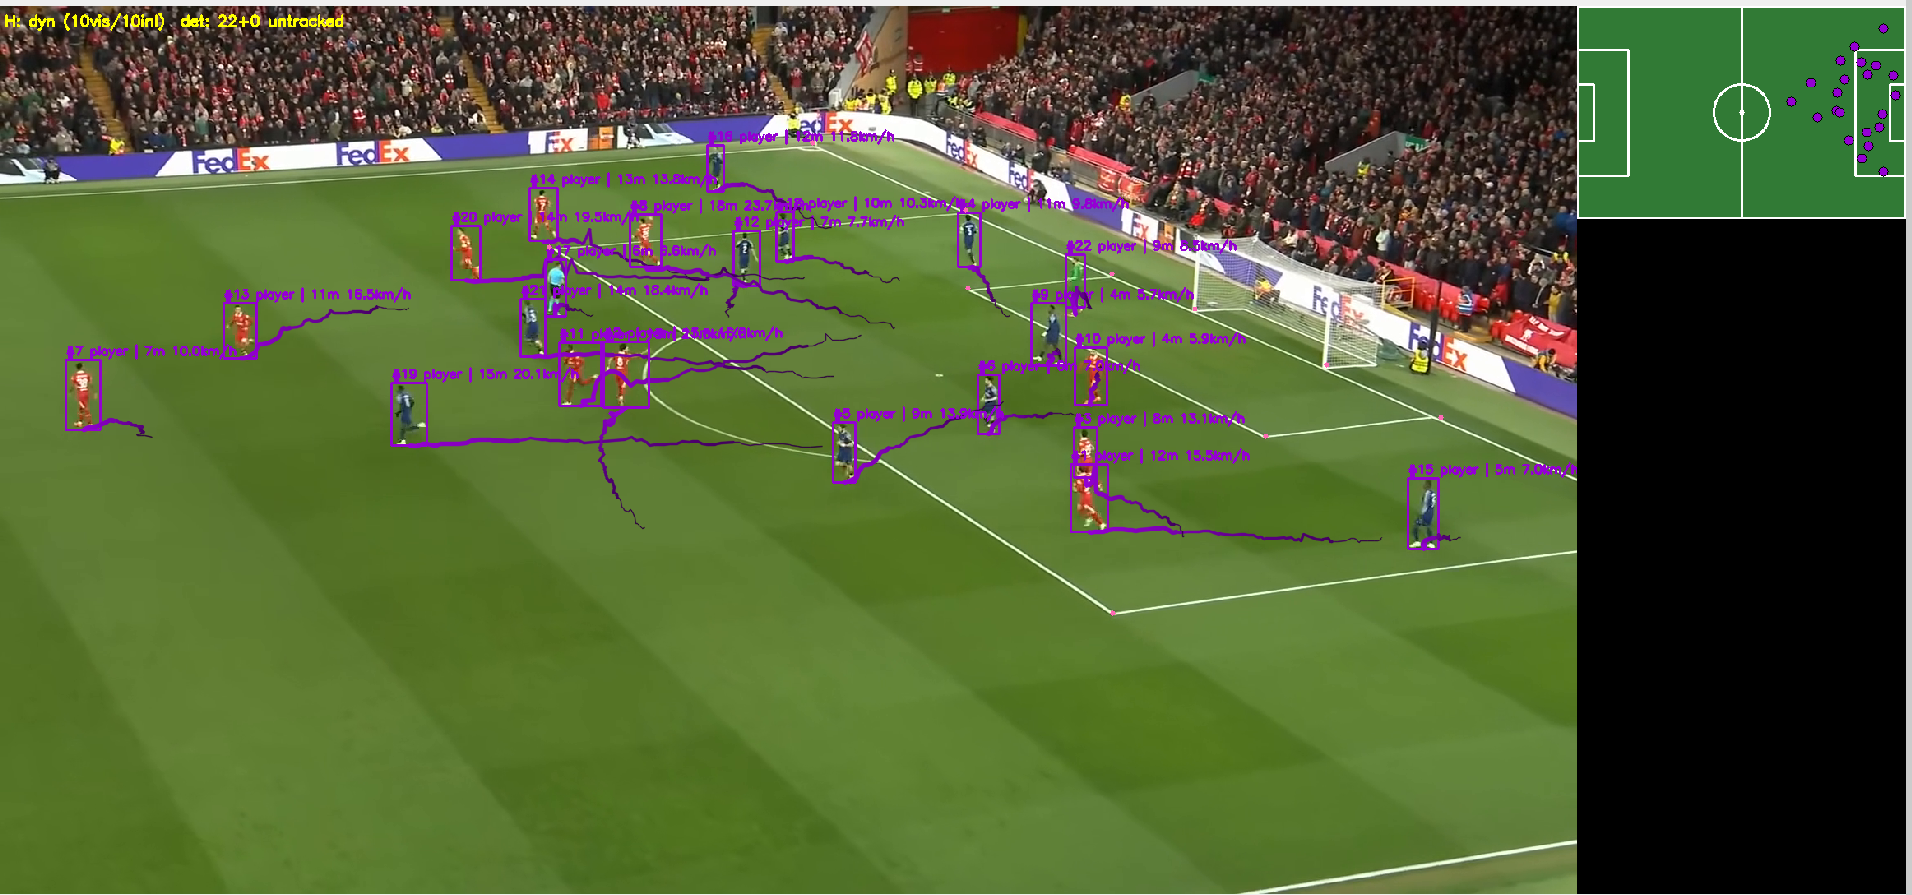
\includegraphics[width=\linewidth]{ex1.png}
  \caption{Ujęcie z dobrą homografią (\texttt{H: dyn, 10 widocznych / 10 inlierów}).
  Widoczne ramki zawodników z numerami ID, dystansem i prędkością, zanikające
  ślady trajektorii oraz minimapa 2D z naniesionymi pozycjami.}
  \label{fig:ex1}
\end{figure}

\begin{figure}[H]
  \centering
  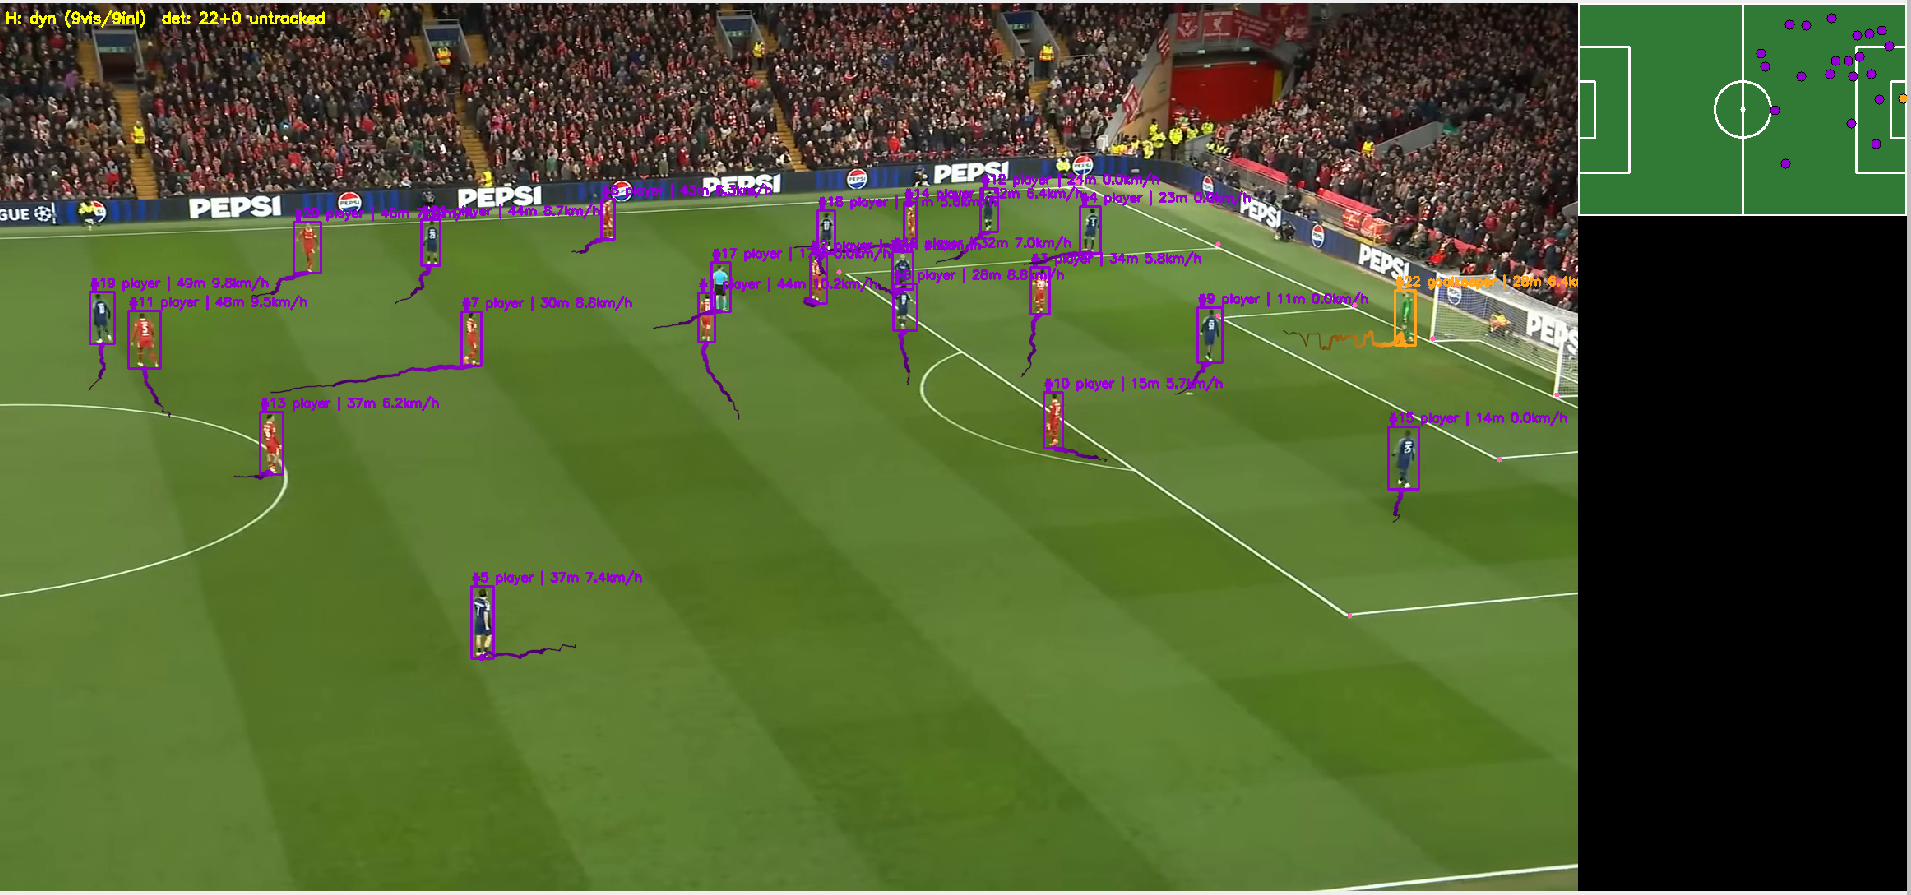
\includegraphics[width=\linewidth]{ex2.png}
  \caption{Inne ujęcie z poprawnie wyznaczoną homografią. Większość zawodników
  ma stabilne ID i wyliczone statystyki; bramkarz po prawej stronie jest
  poprawnie odróżniony (inny kolor ramki).}
  \label{fig:ex2}
\end{figure}

\begin{figure}[H]
  \centering
  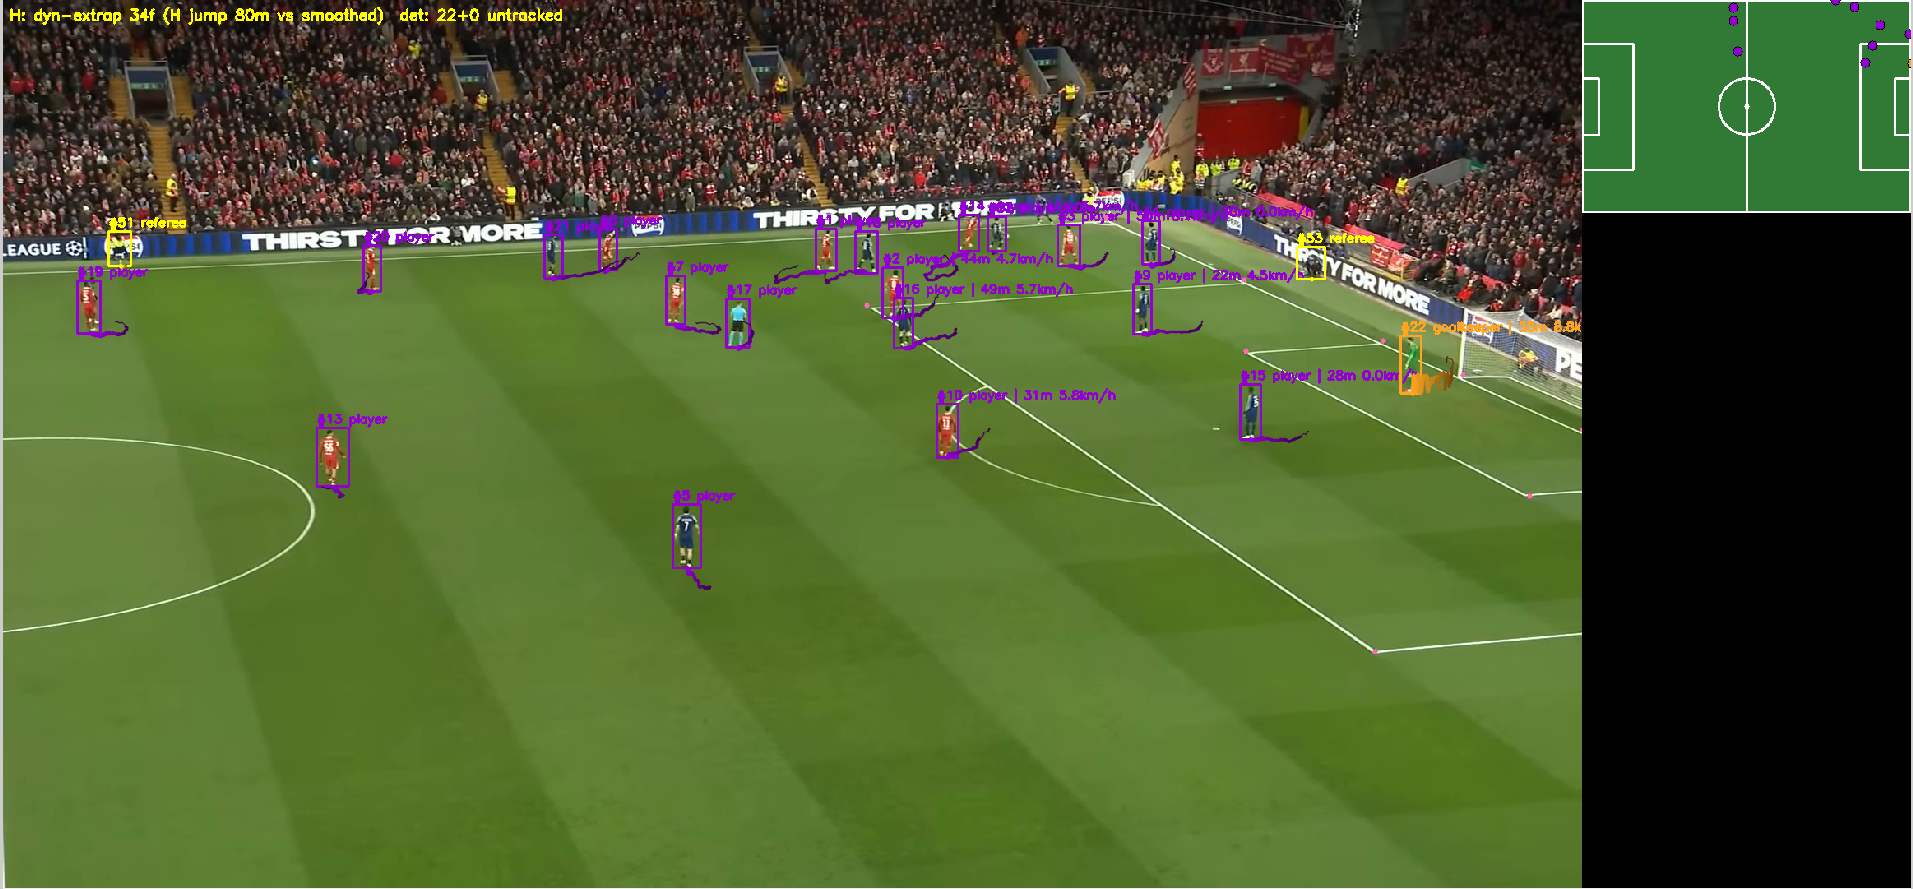
\includegraphics[width=\linewidth]{ex3.png}
  \caption{Ujęcie z ekstrapolowaną homografią (status \texttt{dyn-extrap}). Gdy
  model chwilowo gorzej widzi punkty boiska, utrzymywana jest ostatnia poprawna
  macierz; widać też wykrytego sędziego (oddzielny kolor ramki).}
  \label{fig:ex3}
\end{figure}

\begin{figure}[H]
  \centering
  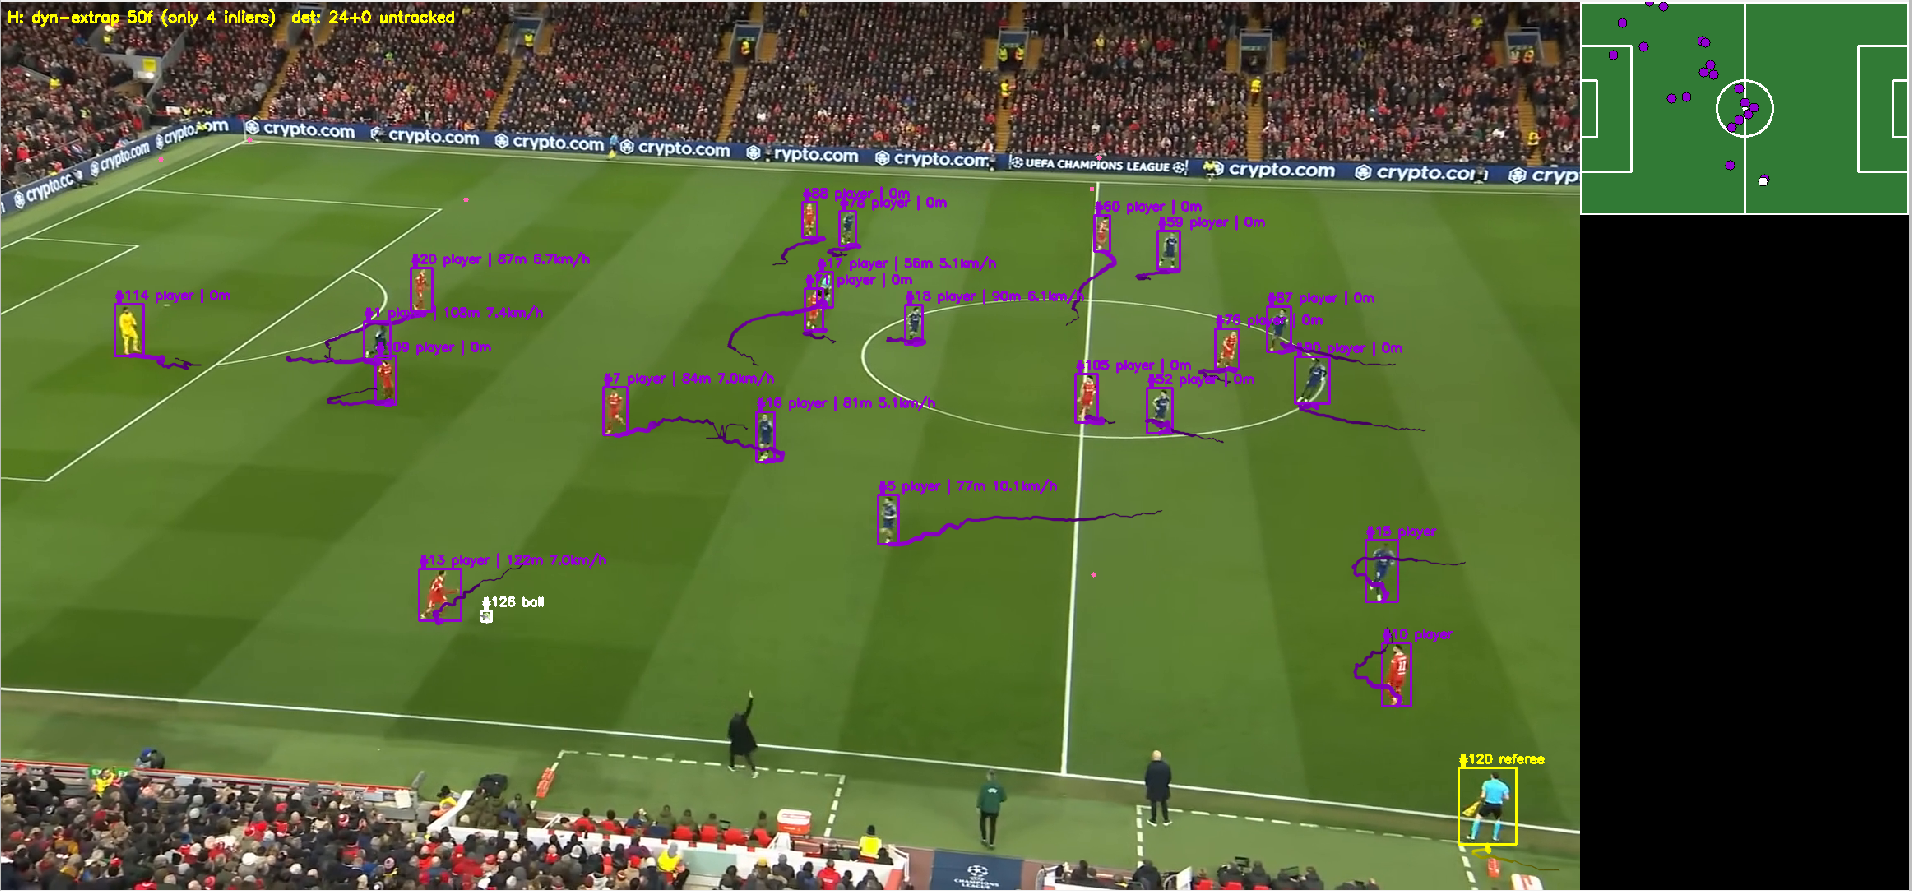
\includegraphics[width=\linewidth]{ex4.png}
  \caption{Szerokie ujęcie z widoczną piłką (\texttt{ball}) i sędzią
  (\texttt{referee}) -- przykład klatki, w której rzadkie klasy zostały wykryte.
  Część etykiet prędkości pokazuje \texttt{0~km/h} dla stojących zawodników.}
  \label{fig:ex4}
\end{figure}

\subsection{Wyniki ilościowe (\texttt{process.py})}

Na potrzeby sprawozdania uruchomiono potok wsadowy na 20-sekundowym fragmencie
(500 klatek, 1920$\times$1080, 25~fps) jednego z klipów z repozytorium,
przy użyciu wytrenowanych modeli \texttt{best.pt} i \texttt{pitch.pt} oraz karty
GPU (CUDA). Tabela~\ref{tab:proc} zawiera podsumowanie wygenerowane przez
\texttt{process.py}.

\begin{table}[H]
\centering
\small
\caption{Podsumowanie uruchomienia \texttt{process.py} (fragment 500 klatek).}
\label{tab:proc}
\begin{tabular}{l r}
\toprule
Metryka & Wartość \\
\midrule
Klatki wejściowe          & 500 \\
Przepustowość             & 7,8 fps \\
Współczynnik czasu rzecz.\ & 0,31$\times$ \\
Homografia zaufana        & 100\% klatek \\
\quad w tym świeże dopasowania & 82\% \\
\quad w tym ekstrapolacja      & 18\% \\
\quad fallback (brak minimapy) & 0\% \\
Unikalne ID zawodników    & 39 \\
Łączny dystans            & 878 m \\
Maks.\ prędkość końcowa   & 11,2 km/h \\
\bottomrule
\end{tabular}
\end{table}

Z analizy zapisanego pliku \texttt{frames.jsonl} (rekord na każdą klatkę) wynika
wyraźna nierównowaga w wykrywalności klas, co potwierdza obserwacje jakościowe.
Tabela~\ref{tab:cls} pokazuje, w jakim odsetku klatek pojawiła się dana klasa
oraz średnią liczbę śledzonych ramek na klatkę.

\begin{table}[H]
\centering
\small
\caption{Wykrywalność klas na fragmencie 500 klatek.}
\label{tab:cls}
\begin{tabular}{l r r}
\toprule
Klasa & Obecna w klatkach & Liczba detekcji (suma) \\
\midrule
player (zawodnik)   & 500 / 500~(100,0\%) & 10\,546 \\
goalkeeper (bramkarz) & 283 / 500~(56,6\%) & 286 \\
referee (sędzia)    & 96 / 500~(19,2\%)   & 108 \\
ball (piłka)        & 55 / 500~(11,0\%)   & 55 \\
\bottomrule
\end{tabular}
\end{table}

Średnio na klatkę przypadały 22 śledzone ramki (maksymalnie 25). Dane te
jednoznacznie potwierdzają, że zawodnicy są wykrywani poprawnie
(w każdej klatce), bramkarze w ponad połowie klatek, natomiast
\textbf{sędziowie i piłka wykrywani są tylko sporadycznie} (odpowiednio ok.~19\%
i 11\% klatek).

\subsection{Stabilność homografii (\texttt{eval.py homography})}

Uruchomiono również ewaluację stabilności homografii na tym samym fragmencie
(co trzecia klatka). Wyniki (Tabela~\ref{tab:homo}) potwierdzają wysoką jakość
dopasowań na ujęciach pokazujących wyraźny fragment boiska.

\begin{table}[H]
\centering
\small
\caption{Wynik \texttt{eval.py homography} (167 przetworzonych klatek).}
\label{tab:homo}
\begin{tabular}{l r}
\toprule
Metryka & Wartość \\
\midrule
Klatki z dopasowaną homografią & 100,0\% \\
Klatki z fallbackiem           & 0,0\% \\
Widoczne punkty (śr.\ $\pm$ odch.) & 8,7 $\pm$ 1,8 \\
Widoczne punkty (min / max)    & 5 / 10 \\
Inliery RANSAC (śr.)           & 7,8 \\
Dryf macierzy klatka-do-klatki (L2) & 0,77 \\
\bottomrule
\end{tabular}
\end{table}

Analiza widoczności poszczególnych punktów pokazała, że na badanym fragmencie
(ujęcie prawej części boiska) punkty prawej strony -- np.\ prawy górny róg
(\texttt{TR}), narożniki prawego pola karnego i bramkowego -- były widoczne w
ok.~100\% klatek, natomiast punkty lewej strony oraz środkowe (koło środkowe,
punkty karne, wierzchołek łuku) w ok.~0\% (są one albo poza kadrem, albo w
ogóle nieobecne w adnotacjach SoccerNet). To wyjaśnia, dlaczego pozycje na
minimapie skupiają się po jednej stronie boiska, gdy kamera kadruje tylko jego
fragment.

\subsection{Co działa, a co nie}

\textbf{Działa dobrze:}
\begin{itemize}[nosep]
  \item detekcja i śledzenie zawodników oraz bramkarzy (trwałe ID, ślady),
  \item wyznaczanie homografii i minimapa 2D na ujęciach z czytelnym boiskiem
        (100\% dopasowań na testowym fragmencie),
  \item wyliczanie dystansu i prędkości (z realistycznymi wartościami i
        wygładzaniem),
  \item generowanie wideo z adnotacjami oraz raportów JSON.
\end{itemize}

\textbf{Ograniczenia:}
\begin{itemize}[nosep]
  \item piłka i sędziowie są wykrywani sporadycznie (mały/szybki obiekt oraz
        położenie na obrzeżach kadru),
  \item przy zbliżeniach na fragment boiska lub przy słabej widoczności linii
        homografia bywa ekstrapolowana, a minimapa rzadsza
\end{itemize}

Istotną przyczyną powyższych niedoskonałości - w szczególności jakości
wykrywania punktów charakterystycznych boiska - były ograniczenia
obliczeniowe po stronie zespołu. Trening modelu boiska jest kosztowny: na
karcie NVIDIA RTX~3090 jedna epoka zajmowała około godziny, co przy
konfiguracji liczącej 60-120 epok i zbiorze augmentowanym liczącym setki
tysięcy obrazów realnie ogranicza liczbę eksperymentów, iteracji
hiperparametrów oraz pełne przeprowadzenie dwuetapowego schematu trenowania
(\texttt{train\_pitch\_partials.py} + \texttt{train\_pitch\_finetune.py})
opisanego w dokumentacji projektu. Przy większych zasobach obliczeniowych
(szybsze GPU, większa pamięć VRAM, możliwość trenowania na pełnym zbiorze
SoccerNet + Roboflow z augmentacją offline) wykrywanie keypointów boiska dałoby
się znacznie poprawić -- m.in.\ przez dłuższy trening, dokładniejsze
dostrojenie na kadry częściowe boiska oraz wyższe metryki keypoint mAP, co
bezpośrednio przekładałoby się na stabilniejszą homografię i wiarygodniejszą
minimapę~2D.

% =====================================================================
\section{Poradnik uruchomieniowy}

\subsection{Instalacja (conda + CUDA)}

Projekt wymaga Pythona w wersji \texttt{>=3.10, <3.13}. Przykładowa instalacja w
środowisku conda z obsługą GPU:

\begin{lstlisting}[style=sh]
conda create -n fbtracker python=3.11 -y
conda activate fbtracker
pip install --upgrade pip
pip install torch torchvision --index-url https://download.pytorch.org/whl/cu124
pip install -e ".[gpu,dev,training]"
# weryfikacja:
python -c "import torch; print(torch.cuda.is_available())"
python scripts/smoke_test.py
\end{lstlisting}

Kluczowe zależności (z \texttt{pyproject.toml}): \texttt{ultralytics} (YOLO26,
trening i wnioskowanie), \texttt{supervision} (ByteTrack), \texttt{lap}
(przypisania), \texttt{opencv-python}, \texttt{numpy}, \texttt{scipy},
\texttt{pandas}, \texttt{pyyaml}, \texttt{matplotlib}, \texttt{plotly},
\texttt{SoccerNet}, \texttt{roboflow}, \texttt{yt-dlp}, \texttt{rich}. Dodatki:
\texttt{gpu} (\texttt{onnx}, \texttt{onnxruntime-gpu}), \texttt{dev}
(\texttt{ruff}, \texttt{pytest}), \texttt{training} (\texttt{albumentations}).
Na systemie Ubuntu przydatne bywają pakiety systemowe:
\texttt{ffmpeg libgl1 libglib2.0-0 libsm6 libxext6}.

\subsection{Najważniejsza uwaga: kodek wideo}

Przykładowe klipy w \texttt{samples/clips/} są zakodowane kodekiem \textbf{AV1},
którego wiele instalacji OpenCV nie potrafi zdekodować (objaw: \texttt{Could not
read first frame}). Przed uruchomieniem warto przekonwertować materiał do
H.264:

\begin{lstlisting}[style=sh]
ffmpeg -i samples/clips/liv_psg_clip1.mp4 -t 20 -c:v libx264 -pix_fmt yuv420p -an clip_h264.mp4
\end{lstlisting}

\subsection{Skrypty uruchomieniowe}

\textbf{\texttt{demo.py}} -- interaktywny podgląd całego potoku w oknie (wymaga
środowiska graficznego). Otwiera wideo lub kamerę, na bieżąco wykrywa, śledzi,
rzutuje na boisko i rysuje minimapę.
\begin{lstlisting}[style=sh]
python demo.py --source clip_h264.mp4 --device cuda
python demo.py --source clip_h264.mp4 --output out.mp4 --no-show   # tryb bezokienkowy
python demo.py --source clip_h264.mp4 --dump                       # zapis JSON na klatke
\end{lstlisting}

\textbf{\texttt{process.py}} -- wsadowe, bezokienkowe przetwarzanie pliku wideo.
Zawsze zapisuje wynikowy film oraz raporty JSON, a na końcu wypisuje tabelę
podsumowującą. To zalecany sposób uzyskania powtarzalnych wyników.
\begin{lstlisting}[style=sh]
python process.py clip_h264.mp4 -o output.mp4 --device cuda
python process.py clip_h264.mp4 --minimal     # tylko ramki + ID + slady
python process.py clip_h264.mp4 --no-minimap --no-analytics
\end{lstlisting}

\textbf{\texttt{eval.py}} -- ewaluacja, czyli pomiar jakości:
\begin{itemize}[nosep]
  \item \texttt{eval.py detector} -- liczy metryki detekcji (mAP, precyzja,
        czułość) detektora na zbiorze walidacyjnym; wymaga lokalnego zbioru
        detekcyjnego. Wynik: \texttt{outputs/reports/eval/detector-*.json}.
  \item \texttt{eval.py pitch} -- liczy metryki modelu boiska (mAP ramki i
        punktów); wymaga lokalnego zbioru boiska. Wynik:
        \texttt{outputs/reports/eval/pitch-*.json}.
  \item \texttt{eval.py homography} -- sprawdza stabilność homografii na
        konkretnym filmie (odsetek dopasowań, powody odrzuceń, widoczność
        punktów); wymaga jedynie wideo i modelu boiska. Wynik:
        \texttt{outputs/reports/eval/homography-*.json}.
\end{itemize}
\begin{lstlisting}[style=sh]
python eval.py homography --source clip_h264.mp4 --stride 3 --device cuda
python eval.py detector --weights models/checkpoints/best.pt --device cuda
python eval.py pitch    --weights models/checkpoints/pitch.pt --device cuda
\end{lstlisting}

\textbf{\texttt{train.py} / \texttt{train\_pitch\_partials.py} /
\texttt{train\_pitch\_finetune.py}} -- trening modeli (opisany w sekcji~5).
\textbf{\texttt{dataset.py}} -- przygotowanie danych (sekcja~\ref{sec:dane}).
\textbf{\texttt{scripts/smoke\_test.py}} -- szybki test poprawności instalacji
(importy modułów, render minimapy, schemat punktów, parsowanie \texttt{--help}
skryptów); nie wymaga modeli, danych ani GPU.

\subsection{Najszybsza weryfikacja działania}

\begin{lstlisting}[style=sh]
conda activate fbtracker
python scripts/smoke_test.py
ffmpeg -i samples/clips/liv_psg_clip1.mp4 -t 20 -c:v libx264 -pix_fmt yuv420p -an clip_h264.mp4
python process.py clip_h264.mp4 -o output.mp4 --device cuda
# wynik: output.mp4 + outputs/reports/demo/<nazwa>-<znacznik_czasu>/summary.json
\end{lstlisting}

% =====================================================================
\section{Podsumowanie}

W ramach projektu zrealizowano kompletny, dwumodelowy potok analizy nagrań
piłkarskich: detektor \texttt{YOLO26-s} rozpoznaje zawodników, bramkarzy,
sędziów i piłkę, tracker ByteTrack nadaje obiektom trwałe identyfikatory, a model
\texttt{YOLO26s-pose} wyznacza 32 punkty charakterystyczne boiska, na podstawie
których liczona jest homografia i budowana minimapa 2D z pozycjami zawodników.
Dodatkowo system wylicza dystans i prędkość zawodników oraz zapisuje
ustrukturyzowane raporty z każdego uruchomienia.

Przeprowadzone testy potwierdziły, że potok działa: na 20-sekundowym fragmencie
homografia była zaufana w 100\% klatek (82\% świeżych dopasowań), wykryto
39~unikalnych identyfikatorów zawodników, a wartości dystansu i prędkości były
realistyczne. Najmocniejszą stroną systemu jest detekcja i śledzenie
zawodników oraz bramkarzy wraz z poprawnym odwzorowaniem ich pozycji na boisku.
Głównymi ograniczeniami są: sporadyczna wykrywalność piłki i sędziów,
zależność jakości minimapy od tego, jak wyraźnie kamera kadruje linie boiska,
oraz ograniczone zasoby obliczeniowe przy treningu modelu keypointów (ok.\
godzina na epokę na RTX~3090), co uniemożliwiło pełne wykorzystanie
dwuetapowego schematu uczenia i ograniczyło dalszą poprawę detekcji punktów
boiska.


\end{document}
